% chapter07.tex

 %%%%%%%%%%%%%%%%%%%%%%%%%%%%%%%%%%%%%%%%%%%%%%%%%%%%%%%%%%%%%%%%%%%%%%%%%%%%%
 %                                                                           %
 %    PyMS documentation                                                     %
 %    Copyright (C) 2005-2010 Vladimir Likic                                 %
 %                                                                           %
 %    The files in this directory provided under the Creative Commons        %
 %    Attribution-NonCommercial-NoDerivs 2.1 Australia license               %
 %    http://creativecommons.org/licenses/by-nc-nd/2.1/au/                   %
 %    See the file license.txt                                               %
 %                                                                           %
 %%%%%%%%%%%%%%%%%%%%%%%%%%%%%%%%%%%%%%%%%%%%%%%%%%%%%%%%%%%%%%%%%%%%%%%%%%%%%

\chapter{The Display module}
\label{chapter:display}
PyMS has graphical capabilities to display information such as ion chromatogram
objects (ICs), total ion chromatogram (TIC), and detected lists of peaks.
This functionality is provided by the package matplotlib, which must be installed
in order to use the Display module and to run the scripts referred to in this
chapter. The instructions for this are provided in \ref{subsec:matplotlib}.

\section{Displaying the TIC}
\label{sec:display-tic}
\noindent
[ {\em This example is in pyms-test/70a} ]

TIC must first be extracted from the data (see section
\ref{sec:ion-chromatogram-object}).  Once the TIC object is created,
a simple call to the function {\tt plot\_ics()} displays the TIC in a
graphical window. In addition to the TIC, two strings may be passed
to plot\_ics() which label the data (in this case 'TIC'), and the
overall plot ('TIC for gc01\_0812\_066').

\begin{verbatim}
>>> plot_ics(tic, 'TIC','TIC for gc01_0812_066')
\end{verbatim}

The window in figure \ref{fig:70a} should now be displayed:

\begin{figure}
  \begin{center}
    \includegraphics[scale=0.33]{graphics/chapter07/test-70a.eps}
  \end{center}
  \caption{Graphics window displayed by the script 70a/proc.py}
  \label{fig:70a}
\end{figure}

To zoom in on a portion of the plot, select the
\includegraphics[scale=0.5]{graphics/chapter07/magnifier_button.eps}
button, hold down the left mouse button while dragging a rectangle over
the area of interest. To return to the original view, click on the
\includegraphics[scale=0.5]{graphics/chapter07/home_button.eps} button.

The 
\includegraphics[scale=0.5]{graphics/chapter07/cross_button.eps}
button allows panning across the zoomed plot. 

\section{Displaying multiple ion chromatogram objects}

\noindent
[ {\em This example is in pyms-test/70b} ]

The Display module can plot multiple ICs and the TIC on the same figure,
as shown in the following example. First, a list of ion chromatogram
objects is created:

\begin{verbatim}
>>> tic = data.get_tic()
>>> ic = im.get_ic_at_mass(73)
>>> ic1 = im.get_ic_at_mass(147)
>>> ics = [tic, ic, ic1]
\end{verbatim}

This list is passed to the function {\tt plot\_ics()}, along with a list
of strings to label each ion chromatogram:

\begin{verbatim}
>>> plot_ics(ics, ['TIC', '73','147'], 'TIC and ICs for m/z = 73 & 147')
\end{verbatim}

This results in figure \ref{fig:70b} being displayed:

\begin{figure}
  \begin{center}
    \includegraphics[scale=0.33]{graphics/chapter07/test-70b.eps}
  \end{center}
  \caption{Graphics window displayed by the script 70b/proc.py}
  \label{fig:70b}
\end{figure}

\section{Displaying the mass spectrum}
[ {\em This example is in pyms-test/70c} ]

The pyms Display module can also be used to display individual mass spectra. The 
following selects the mass spectrum of interest:

\begin{verbatim}
... im is an intensity matrix
>>> ms = im.get_ms_at_index(1024)
\end{verbatim}

The pyms function {\tt plot\_ms()} can then be called to display the mass spectrum to 
the screen.

\begin{verbatim}
>>> plot_ms(ms, 'Mass Spectrum at index 1024')
\end{verbatim}

The resulting window is shown below in figure \ref{fig:70c}

\begin{figure}
  \begin{center}
    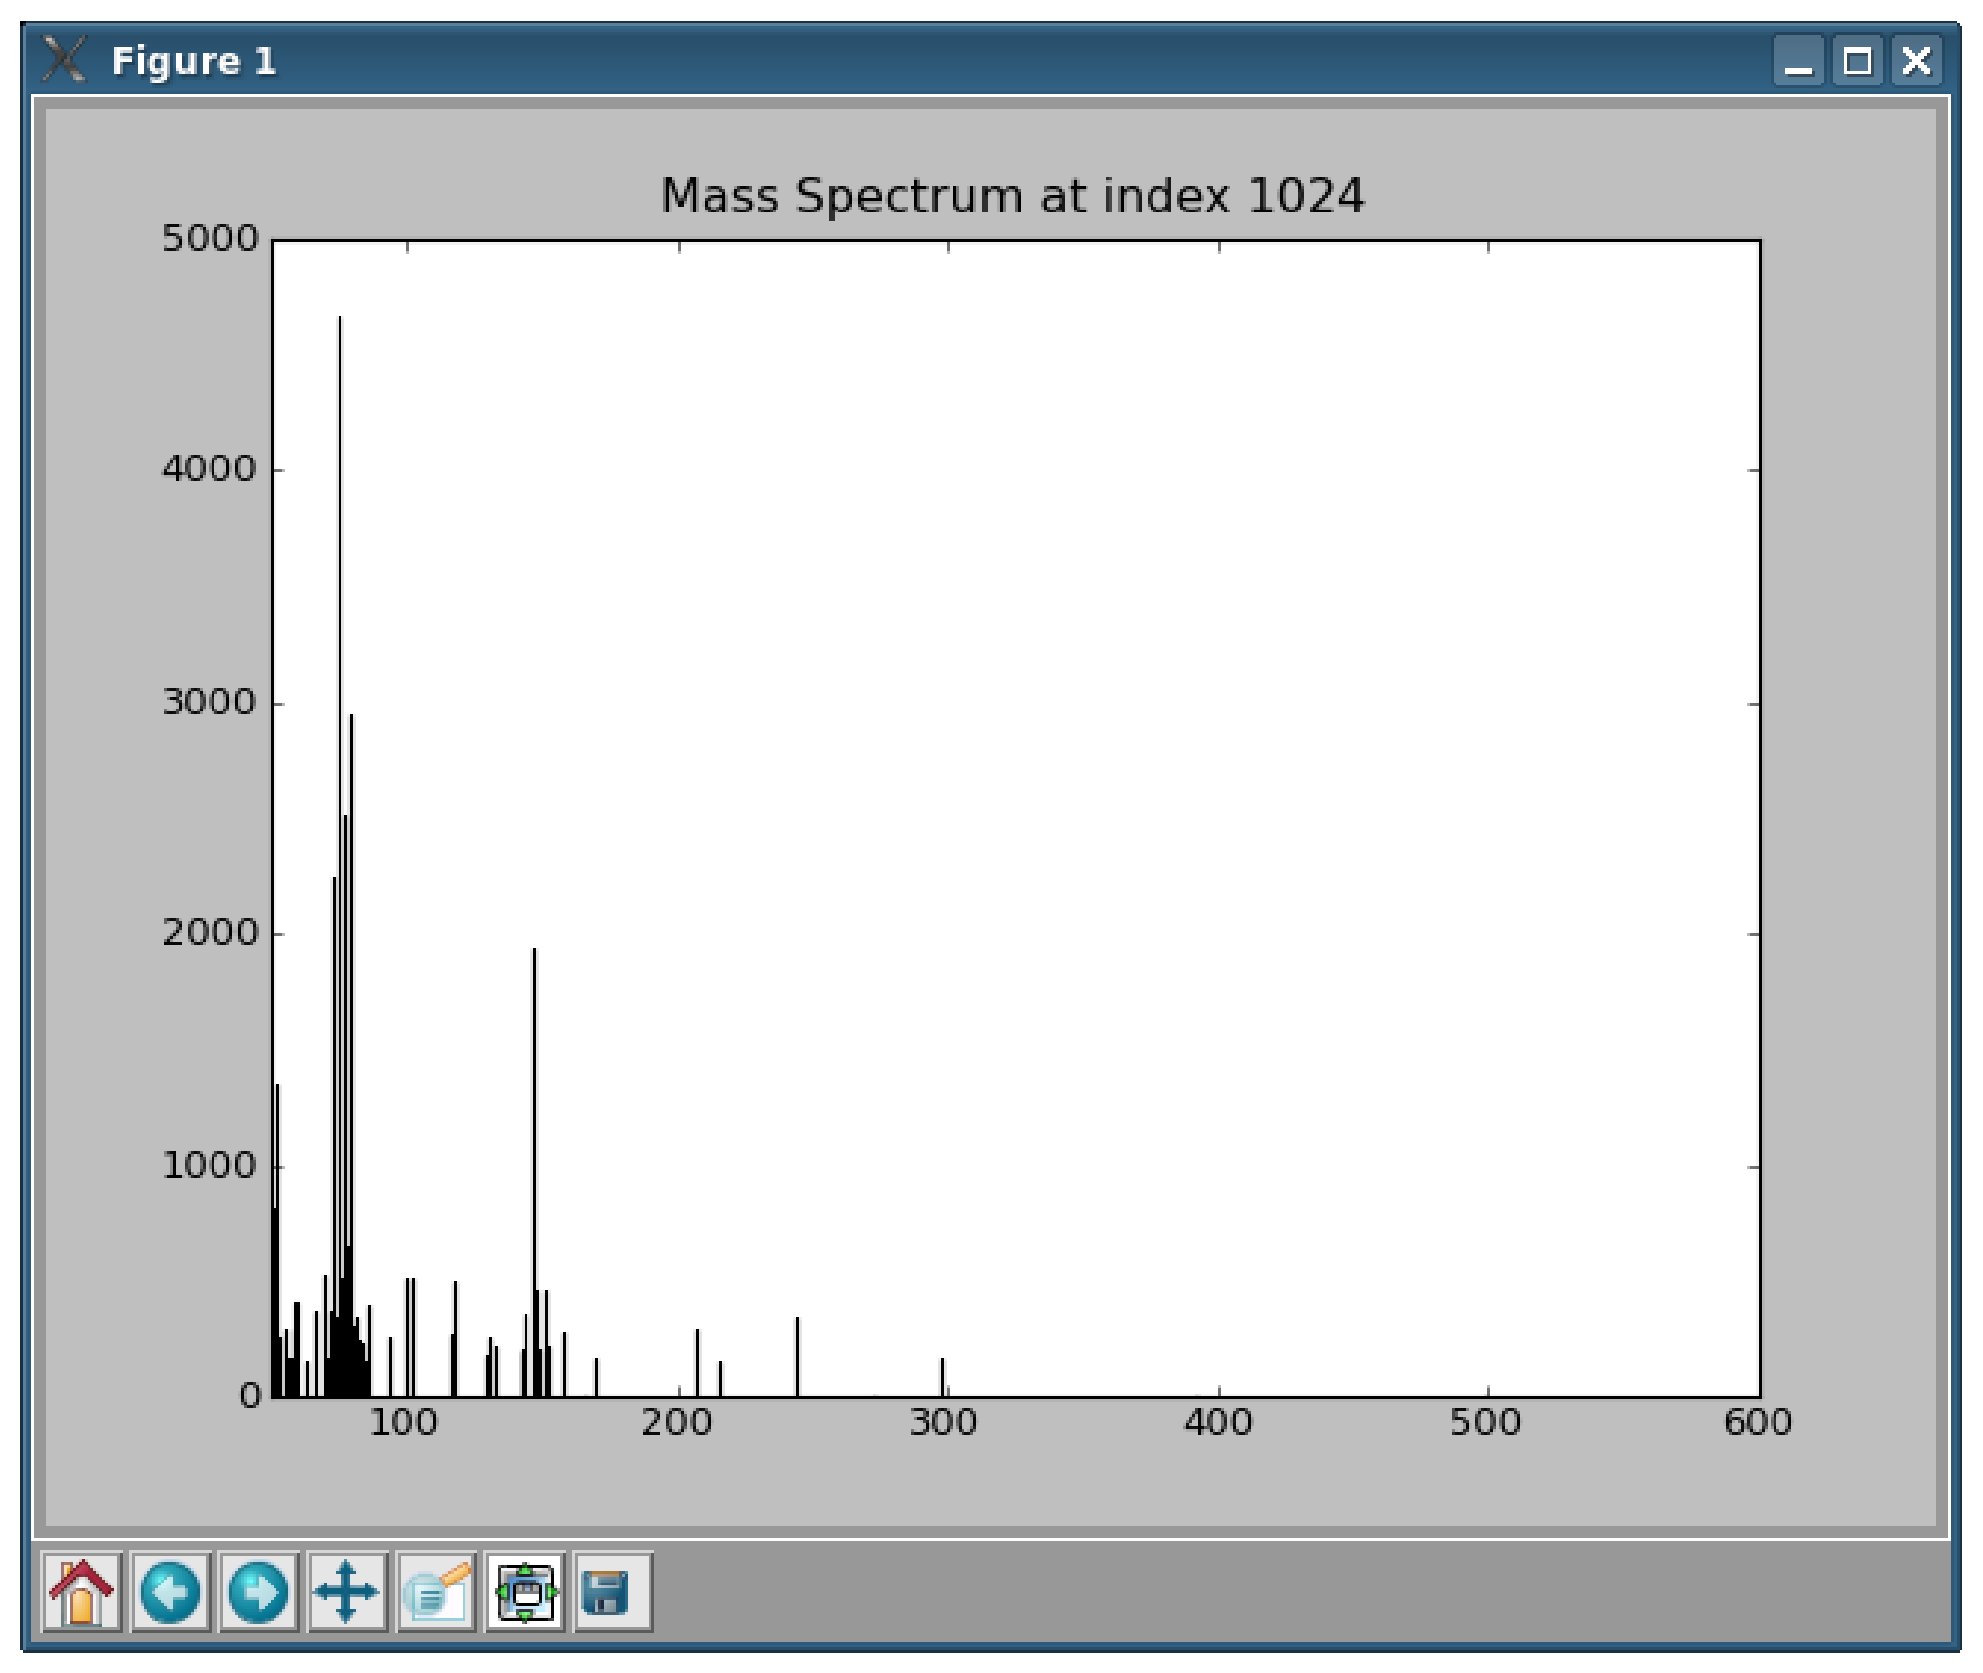
\includegraphics[scale=0.33]{graphics/chapter07/test-70c.eps}
  \end{center}
  \caption{Graphics window displayed by the script 70c/proc.py}
  \label{fig:70c}
\end{figure}

\section{Displaying detected peaks on the TIC plot}

\noindent
[ {\em This example is in pyms-test/71} ]

The Display class is a more powerful implementation of plotting which 
allows plotting of detected peaks and user interaction with the plot
figure.

In order to plot a list of peaks, the peaks must be created first.
The example pyms-test/71 contains the script {\tt proc\_save\_peaks.py}
which produces such a peak list. For more information on detecting peaks
see section \ref{sec:peak-detection}. The function {\tt store\_peaks()}
in {\tt proc\_save\_peaks.py} stores the peaks, while {\tt load\_peaks()}
in {\tt proc.py} loads them for the Display class to use.

When using the Display Class, a series of plots is added to the figure
one at a time before the final plot is displayed. The first step is
always creating an instance of the Display class:

\begin{verbatim}
>>>display = Display()
\end{verbatim}

Next some ics and the TIC are plotted. Unlike in simple plotting, the
TIC is plotted using a separate function. This function ensures that
the TIC is always plotted in blue for easy reference. The legend for
each IC is supplied to the functions, but the overall figure label
is not supplied at this time.

\begin{verbatim}
>>> display.plot_ics(ics, ['73','147'])
>>> displat.plot_tic(tic, 'TIC')
\end{verbatim}

The function {\tt plot\_peaks()} adds the PyMS detected peaks to the
figure.

\begin{verbatim}
>>>display.plot_peaks(peak_list, 'Peaks')
\end{verbatgoogle.com.au/im}

Finally, the function {\tt do\_plotting()} is called to draw the figure with 
labels and display the plot.

\begin{verbatim}
>>> display.do_plotting('TIC, ICs, and PyMS Detected Peaks')
\end{verbatim}

This should result in figure \ref{fig:71-ics} being displayed:

\begin{figure}
  \begin{center}
    \includegraphics[scale=0.33]{graphics/chapter07/test-71-ICs.eps}
  \end{center}
  \caption{Graphics window displayed by the script 71/proc.py}
  \label{fig:71-ics}
\end{figure}

\subsection{User interaction with the plot window}

When using the Display class, the resulting figure window can be used to
access data about the displayed peaks.

Clicking on a peak causes a list of the 5 highest intensity eluting ions
at that peak to be written to the screen in order.  Clicking a mouse
 button over one of the peaks should result in output similar to the
following:

\begin{verbatim}
>>> mass     intensity
>>> 273     1003678.47619
>>> 73      625396.428571
>>> 147     526953.333333
>>> 363     255903.714286
>>> 347     241031.333333
\end{verbatim}

In addition, clicking a mouse button other than the left button on a peak
displays the mass spectrum at the peak in a new window (figure \ref{fig:71-spec}):

\begin{figure}
  \begin{center}
    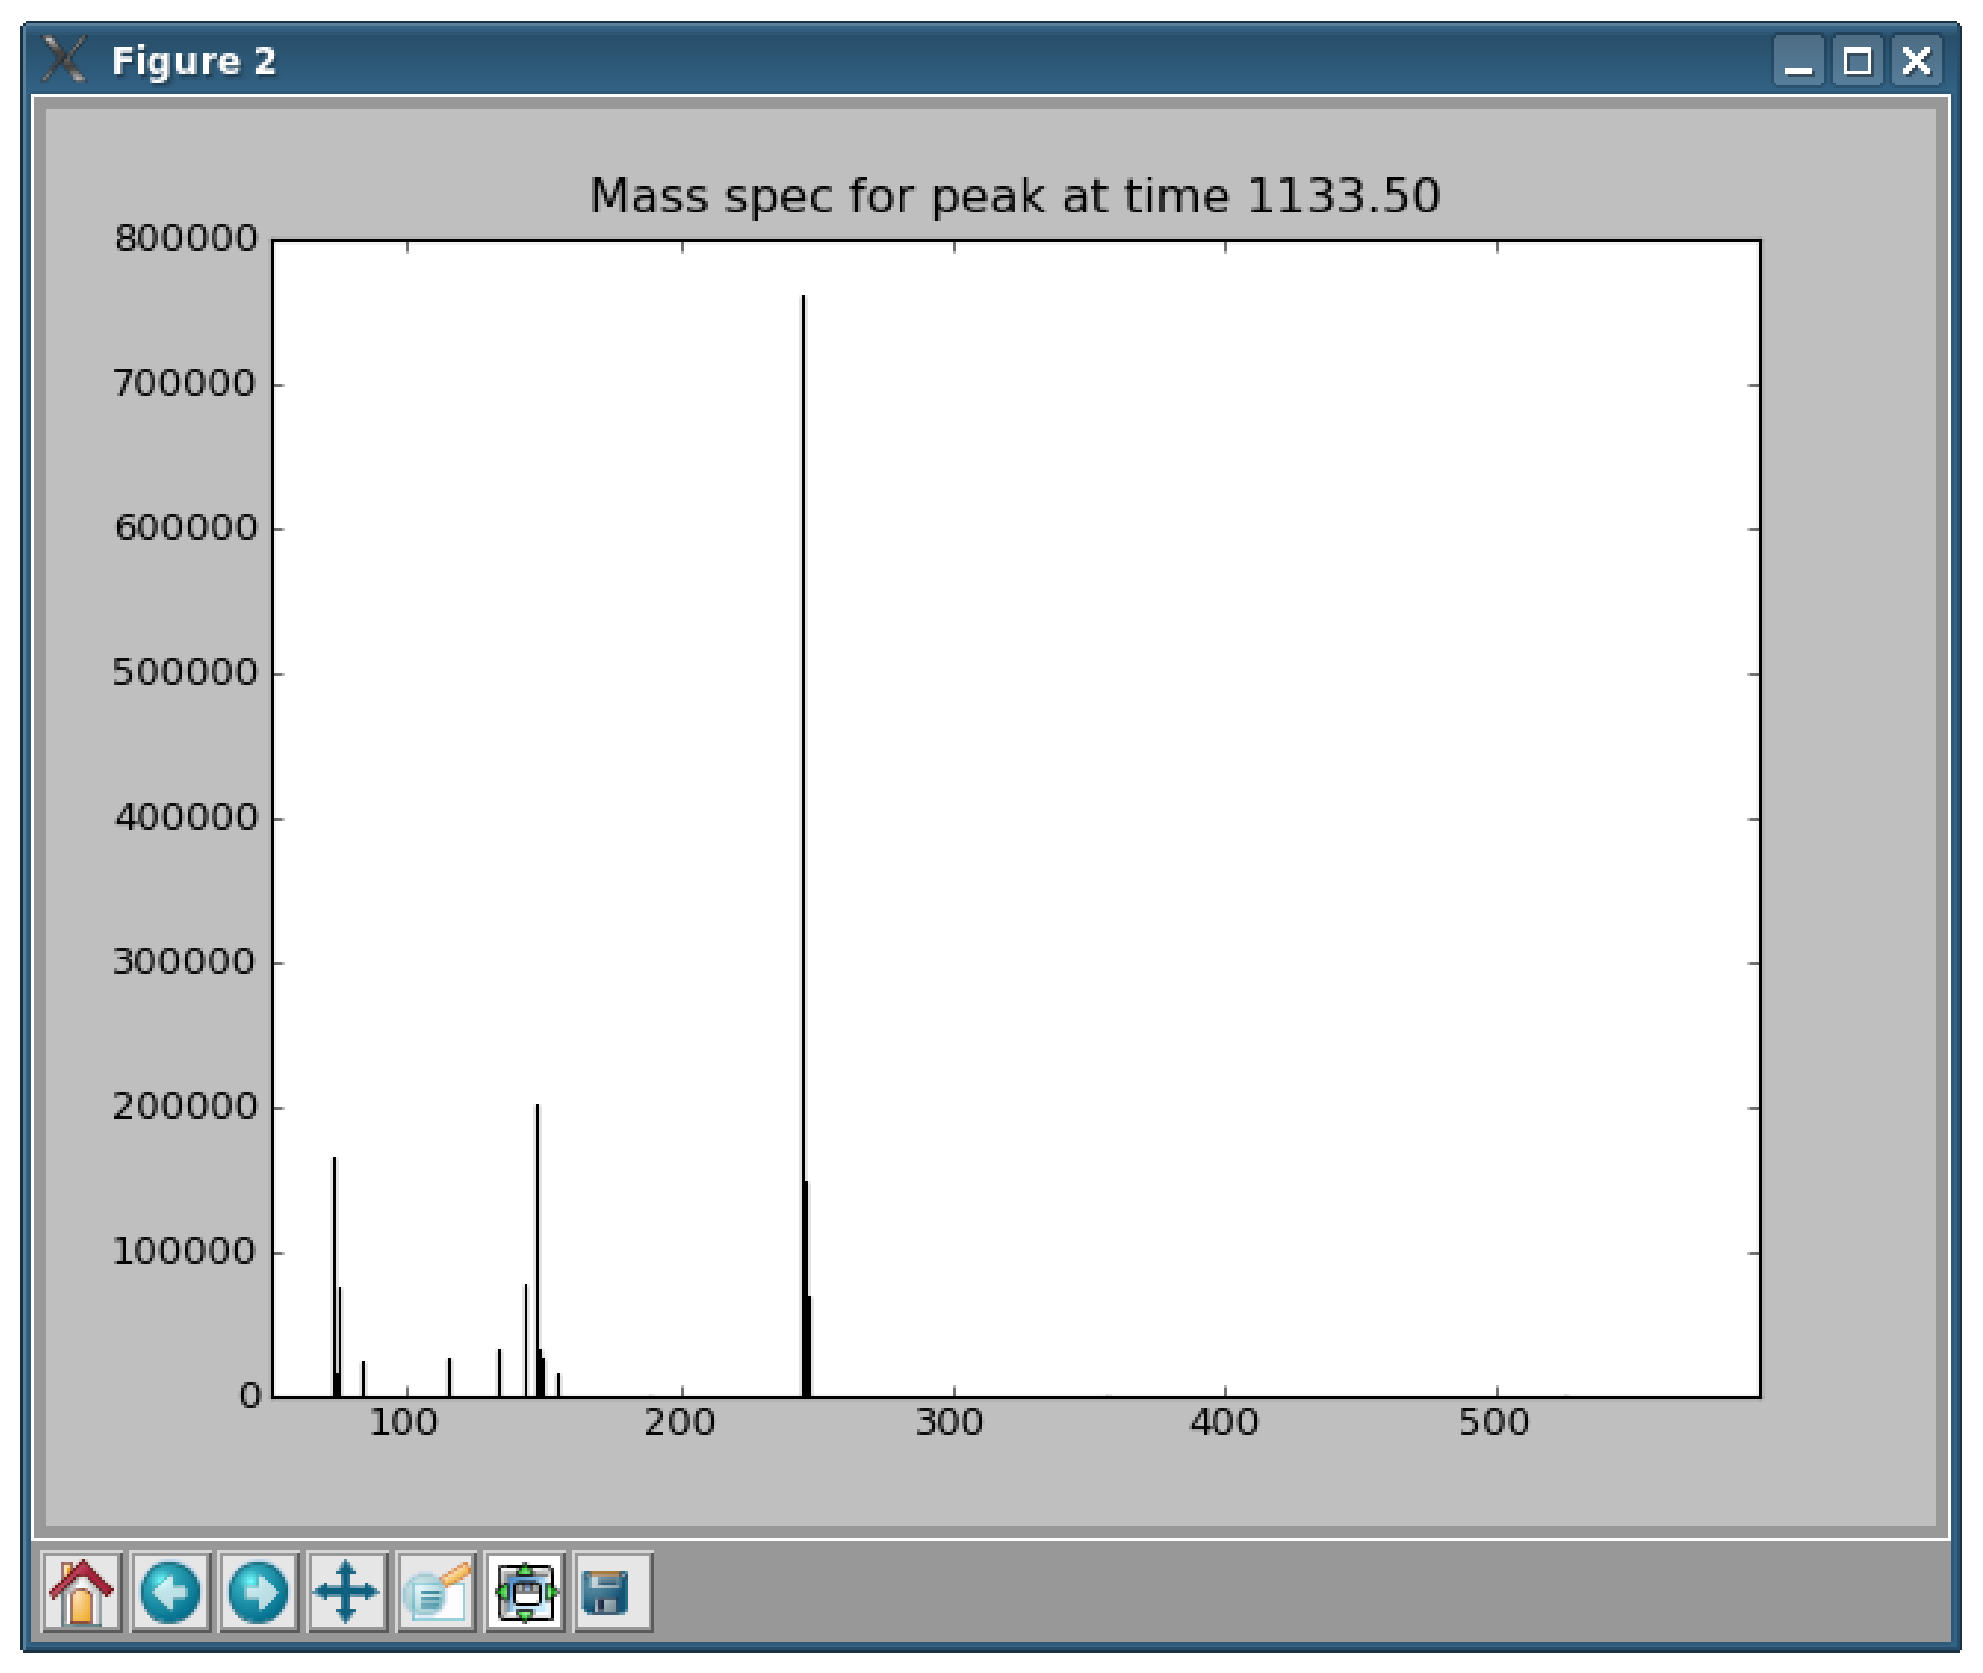
\includegraphics[scale=0.33]{graphics/chapter07/test-71-spec.eps}
  \end{center}
  \caption{The mass spectrum displayed by PyMS when a peak in the
  graphics window of Figure \ref{fig:71-ics} is clicked on}
  \label{fig:71-spec}
\end{figure}

Clicking on other peaks will display further mass spectrums for those peaks
in new windows.

